\section{Hilbert空间}
\label{sec:ipspace-hilbert-spaces}

内积空间是赋范空间，因而可以谈柯西列与完备性。下一节之后的最佳逼近与无限展开都要从柯西列得到极限，所以需要把完备性与内积放在一起。

\begin{definition}[Hilbert空间]
\label{def:ipspace-hilbert}
若内积空间在诱导范数下完备，即诱导度量满足第~\ref{chap:metric-spaces}章的完备性，称它为\term{Hilbert空间}（Hilbert space）。
\end{definition}

按定义，Hilbert空间就是范数来自内积的Banach空间。反过来不成立：上一节说明一致范数与$L^1$范数不满足平行四边形恒等式，而第~\ref{chap:normed-spaces}章证明了$C[0,1]$在一致范数下完备、$L^1[0,1]$完备，所以它们是Banach空间，却不是Hilbert空间。“有没有内积”和“是否完备”是两个独立的判断。

有限维内积空间总是完备的，因为有限维赋范空间在任意范数下都完备。所以有限维时，内积空间与Hilbert空间是同一回事，卷二的全部正交理论都在完备空间中进行。无限维时，完备性要对每个具体空间单独证明；下面两个例子说明它确实可能不成立。

\paragraph{有限支撑数列}
在$c_{00}$上取内积$\langle x,y\rangle=\sum_k\overline{x_k}y_k$。令
\begin{equation*}
x^{(N)}=(1,\tfrac12,\ldots,\tfrac1N,0,0,\ldots)\in c_{00}.
\end{equation*}
对$M>N$，
\[
 \lVert x^{(M)}-x^{(N)}\rVert^2=\sum_{k=N+1}^M\frac1{k^2}\leq\sum_{k>N}\frac1{k^2}\to0,
\]
所以$(x^{(N)})$是柯西列。

它在$c_{00}$中没有极限。若$\lVert x^{(N)}-y\rVert\to0$对某个$y\in c_{00}$成立，由于每个坐标的差都不超过范数，$\lvert x^{(N)}_k-y_k\rvert\leq\lVert x^{(N)}-y\rVert$，每个坐标都收敛，所以$y_k=\lim_Nx^{(N)}_k=1/k$对所有$k$成立。这样的$y$有无穷多项非零，不在$c_{00}$中，矛盾。所以$c_{00}$是不完备的内积空间。

\paragraph{连续函数与平方积分}
在$C[-1,1]$上取实内积$\langle f,g\rangle=\int_{-1}^1fg\,dx$，诱导范数记为$\lVert\cdot\rVert_2$。连续斜坡
\[
 g_n(x)=\begin{cases}-1,&x\leq-1/n,\\ nx,&\lvert x\rvert<1/n,\\ 1,&x\geq1/n\end{cases}
\]
越来越陡，越来越像符号函数$\operatorname{sgn}$，如图~\ref{fig:ipspace-ramp-step}所示。对$m>n$，两函数只在$\lvert x\rvert<1/n$上不同且差的绝对值不超过$1$，所以$\lVert g_n-g_m\rVert_2^2\leq2/n$，$(g_n)$是柯西列。

\begin{figure}[!htb]
  \centering
  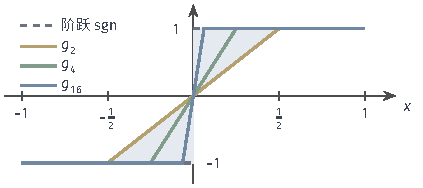
\includegraphics[width=71.6mm]{figures/02-abstract-mathematics/03-function-spaces/tikz/c1-ramp-step/figure.pdf}
  \caption{连续斜坡$g_n$逼近符号函数$\operatorname{sgn}$。$g_n$在$\lvert x\rvert\geq1/n$处与$\operatorname{sgn}$相同，只在宽为$2/n$的区间内线性过渡；阴影是$n=2$时二者之差所在的区域。直接积分得$\int_{-1}^1(g_n-\operatorname{sgn})^2\,dx=\tfrac{2}{3n}\to0$，但$\operatorname{sgn}$在$0$处跳跃，没有连续代表。}
  \label{fig:ipspace-ramp-step}
\end{figure}

它在$C[-1,1]$中没有$\lVert\cdot\rVert_2$极限。若连续函数$g$满足$\lVert g_n-g\rVert_2\to0$，任取$\delta\in(0,1)$，当$n>1/\delta$时$g_n$在$[\delta,1]$上恒为$1$，于是$\int_\delta^1(1-g)^2\,dx\leq\lVert g_n-g\rVert_2^2\to0$，由连续性$g=1$在$[\delta,1]$上成立；同理$g=-1$在$[-1,-\delta]$上成立。$\delta$任意，$g$在$0$处不可能连续，矛盾。这与第~\ref{chap:normed-spaces}章积分范数下的不完备例子是同一机制，只是误差改用平方累计。

两个例子中，柯西列的“极限”都存在，只是不在原来的集合里：前者是平方可和的数列$(1/k)$，后者是平方可积的阶跃函数。下一节的$\ell^2$与$L^2$正是把这些极限都收进来的空间。
